% CVPR 2022 Paper Template
% based on the CVPR template provided by Ming-Ming Cheng (https://github.com/MCG-NKU/CVPR_Template)
% modified and extended by Stefan Roth (stefan.roth@NOSPAMtu-darmstadt.de)

\documentclass[10pt,twocolumn,letterpaper]{article}

%%%%%%%%% PAPER TYPE  - PLEASE UPDATE FOR FINAL VERSION
%\usepackage[review]{cvpr}      % To produce the REVIEW version
\usepackage{cvpr}              % To produce the CAMERA-READY version
%\usepackage[pagenumbers]{cvpr} % To force page numbers, e.g. for an arXiv version

% Include other packages here, before hyperref.
\usepackage{graphicx}
\usepackage{amsmath}
\usepackage{amssymb}
\usepackage{booktabs}
\usepackage{graphicx}
\usepackage{caption}
\usepackage{float}
\usepackage{dblfloatfix}
\usepackage{tabularx}
\usepackage{array}
\newcolumntype{L}{>{\centering\arraybackslash}m{1.5cm}}


% It is strongly recommended to use hyperref, especially for the review version.
% hyperref with option pagebackref eases the reviewers' job.
% Please disable hyperref *only* if you encounter grave issues, e.g. with the
% file validation for the camera-ready version.
%
% If you comment hyperref and then uncomment it, you should delete
% ReviewTempalte.aux before re-running LaTeX.
% (Or just hit 'q' on the first LaTeX run, let it finish, and you
%  should be clear).
\usepackage[pagebackref,breaklinks,colorlinks]{hyperref}


% Support for easy cross-referencing
\usepackage[capitalize]{cleveref}
\crefname{section}{Sec.}{Secs.}
\Crefname{section}{Section}{Sections}
\Crefname{table}{Table}{Tables}
\crefname{table}{Tab.}{Tabs.}


%%%%%%%%% PAPER ID  - PLEASE UPDATE
\def\cvprPaperID{00002} % *** Enter the CVPR Paper ID here
\def\confName{CVPR}
\def\confYear{2024}


\begin{document}

%%%%%%%%% TITLE - PLEASE UPDATE
\title{Using Fine Tuning to Develop A Modern CNN for CIFAR-10 Dataset}

\author{Brian Drake\\
University of Adelaide\\
THE UNIVERSITY OF ADELAIDE
5005 AUSTRALIA\\
{\tt\small brian.drake@student.adelaide.edu.au}
% For a paper whose authors are all at the same institution,
% omit the following lines up until the closing ``}''.
% Additional authors and addresses can be added with ``\and'',
% just like the second author.
% To save space, use either the email address or home page, not both
}
\maketitle

%%%%%%%%% ABSTRACT
\begin{abstract}
This study investigates the performance of Convolutional Neural Networks (CNNs) for image classification on the CIFAR-10 dataset. The models tested include a baseline model, as well as fine-tuned versions of ResNet50, EfficientNet B0, and VGG16. The improved model, which integrates features from the aforementioned architectures, achieved the best results. After 10 epochs, it reached a training accuracy of 92.77\% and a test accuracy of 79.59\%, with an error rate of 20.41\%. Training was extended to 50 and 100 epochs, leading to improvements in training accuracy, 98.82\%, but a decline in test accuracy 81.95\% at 100 epochs, indicating potential overfitting. Comparison with other models showed that the EfficientNet model achieved a test accuracy of 82.73\%, while ResNet50 and VGG16 demonstrated lower performance. This study highlights the effectiveness of combining transfer learning with architectural innovations from VGG, ResNet, and EfficientNet to develop a more efficient and accurate image classification model, with room for further optimization through regularization techniques and hyperparameter tuning.
\end{abstract}

%%%%%%%%% BODY TEXT
\section{Introduction}
\label{sec:intro}
The CIFAR-10 dataset is a historically established computer vision dataset used for object recognition. Comprised of 60,000 32x32 pixel colour images distributed evenly across 10 classes. These classes are mutually exclusive and do not overlap \cite{cifar10}. This dataset is primarily used for experiments in computer vision.

Computer vision is achieved via Convolutional Neural Networks (CNN), using a CNN model can enable these images can be identified and classified. CNNs are a specific type of multilayer neural network based on living vision. A traditional CNN is comprised of a single or even multiple blocks of convolutional layers and pooling layers. Convolution layers are matrix multiplications that scan over the image grid, allowing for interpretation of visual data. While pooling layers are subsampling layers that reduce the complexity of matrix by reducing it to either the maximum value or average value of the kernel specified. After which a fully connected layer, a layer of perceptron nodes, then interprets that data non-linearly before passing the data through an output layer \cite{recent_trends}. Resulting in a model that can learn what categories of data "look like" and then classify them. While this is an established field in computer vision, machine learning, and artificial intelligence, problems remain in computational time, load, and accuracy. 

Breakthrough models like the VGG \cite{original_vgg}, ResNet \cite{original_resnet}, and EfficientNet \cite{original_efficientnet}, families of models have been made available after learning. Once the model weights have been stored after training, they can be retrieved to either be used directly or fine tuned for a new purpose. Fine tuning enables for previous learning that may be related to the current problem be used to accelerate feature extraction and reduce learning time. Through the study of these fine tuned models their architecture can be used to optimise a simple model into an improved deep bespoke model.  


\section{Method}
\label{sec:method}
A fundamental student model was developed using computer vision techniques. this involved the use of multiple 2D Convolutionl, Batch Normalisation, Max Pooling, and Dense layers, as well as the incorporation of Dropout.

Convolutional layers are a mathematical process whereby primarily image data is processed to extract features such as edges, textures, and shapes. A layer applies small filters (kernels), which are matrices of learnable weights across the input image. Each filter slides, or convolves, across the entire image. At each position a dot product is calculated between the filter and the covered cell of the image matrix. Resulting in a single output value which forms part of the new matrix called a feature map. Multiple layers are applied to create multiple feature maps designed to capture different aspects of the input image. The output is typically passed through a non-linear activation function like ReLu, to introduce non-linear learning assisting in learning complex patterns. Further, in general the more convolution layers added the more complex features a network can learn. Padding refers to the space outside of the input matrix itself where a kernel will apply, this data can be filled in in multiple ways depending on the networks needs. A padding of "same" projects the nearest number in the matrix over the edge to reduce impact on the convolution calculation itself \cite{convolutiontheory}. An example of this entire process can be seen in figure \ref{fig:Convolution example}, where the second cell of a 2D convolution with a 3x3 filter and 'same' padding can be seen. 

\begin{figure} [h]
    \centering
    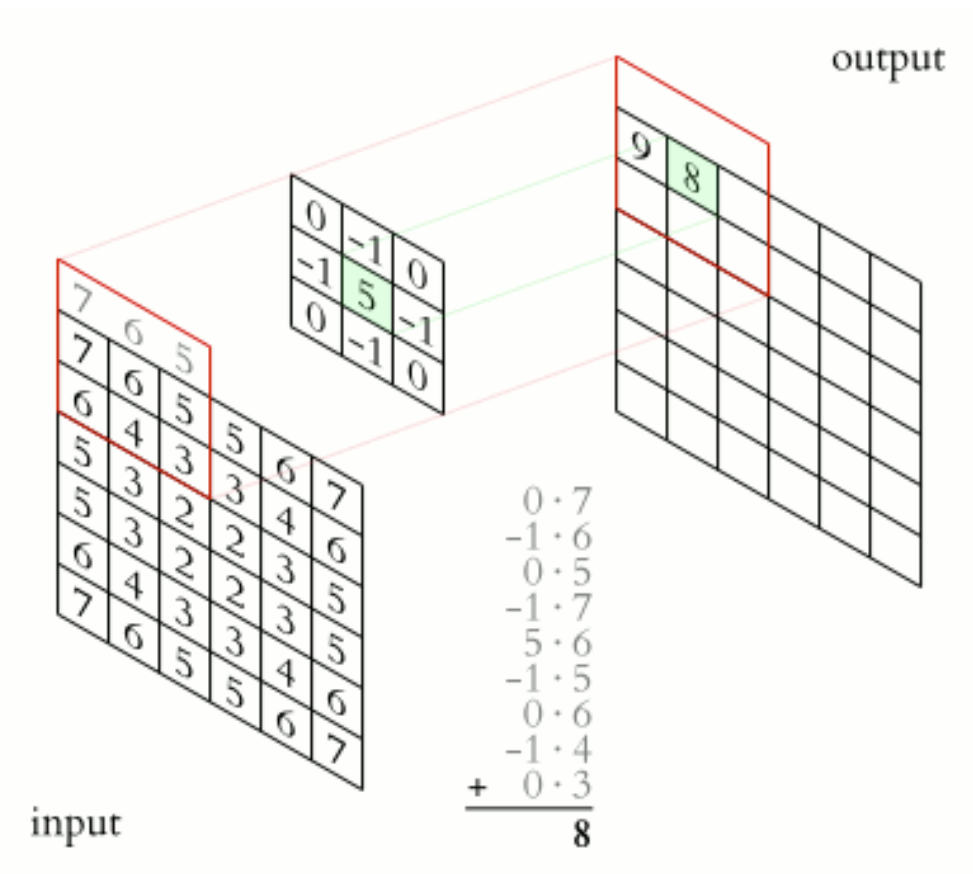
\includegraphics[width=\linewidth]{convolution.png}
    \caption{An example of a 2D convolution \cite{convolutiondiagram}}
    \label{fig:Convolution example}
\end{figure}

Batch Normalisation is a function used where inter-layer outputs of a neural network are transformed to maintain a mean of approximately 0 and a standard deviation of approximately 1 \cite{pytorch}. Enabling faster computation due tot he outputs being smaller. This combats exploding gradient problems and enables epochs to resolve faster. This is represented mathematically as:

\[y = \frac{x-E[x]}{\sqrt{Var[x]+\epsilon}} * \gamma + \beta\]

Where the mean and standard deviation are calculated per-dimension, with and being learnable parameter vectors of size C. C equal to the number of features or channels of the input. 

Max Pooling is a down sampling layer used within CNNs. This reduces spatial dimensions (width and height) of the input feature maps, while retaining the most important information. This operation works similarly to a convolution where a kernel is slid over the matrix and the maximum value is taken within that region. Allowing the network to retain critical information about features while reducing computational load \cite{recent_trends}. By reducing the spatial size and therefore the resolution of the feature map the model in tandem becomes more robust toward small translations or distortions in the input data. This also in turn acts as a form of regularisation and mitigates some overfitting. 

Dense layers are vital in machine learning. They are fully connected nodes that contain activation functions, the aim of which is to interpret mathematically any data given. Typically these are individual perceptron nodes responsible in finding linear separations in highly dimensional data \cite{pytorch}. 

Dropout is a functional layer where during training of the nueral network some elements of the input tensor are randomly changed to zeroes. Achieved as an independant probability, as specified int he architecture, that each node is changed \cite{pytorch}. Depending on the model different probabilities can be passed and mutiple occurences of dropout can be used. The aim of which is to improve regularisation of data dn preventing the co-adaptation of individual nodes \cite{hinton2012improvingneuralnetworkspreventing}. Meaning that increased complexity of the model will be less liekly to create redundant or silent nodes. In turn allwoing for greater generalisation on new data. 

\subsection{VGG16}
VGG16 is one of a family of deep convolutional neural network created by the Visual Geometry Group (VGG) at Oxford. It is characteristic of having 16 layers, 13 convolutional and 3 fully connected. The convolutional layers use a 3x3 kernel with a stride of 1 and 'same' padding to maintain spatial resolution. VGG16 also stacks multiple convolutional layers, 2-3 consecutively, followed by a max pooling layer. The network ends with three fully connected perceptron layers which handle high level features extracted by the previous layer \cite{original_vgg}. This is a straight forward architecture that can extract features but due to its depth and fully connected layers requires large computational input, memory, and needs a strict learning rate when training. 

\subsection{ResNet50}
ResNet50 is the 50 layer version of the ResNet deep convolutional nueral networks that introduced residual learning to address the vanishing gradient problems that have arisen alonside deep networks. ResNet contribution to computer vision is the residual connections, which allow the network to learn "residual" functions rather than tryin to learn the full mapping. Allowing for simplification of optimising deep networks. This is achieved taking an initial convolution before the convolution block begins then adding those back at the end of the block. Creating a shortcut for the block in feature extraction. The 50 layer architecture also featured a bottleneck design where the kernel will be 1x1 then 3x3 then 1x1 again in a convolution block. Further instead of multiple dense layer, ResNet uses a global average pooling, to futher reduce computational parameters \cite{original_resnet} \cite{finetuningresnet50}. This enables ResNet50 to be highly efficient and maintain accuracy even in deep architectures, however requiring more careful implementation and interpretation. 

\subsection{EfficientNet}
EfficientNet is a family of models designed around the use of a compound scaling method to balance depth, width and resolution of a neural network. Achieving higher accuracy with fewer parameters. The chosen EfficientNet model was B0, the simplest and first of the family. Presenting the Inverted Bottleneck Block where, similar to MobileNetV2, the convolution blocks start at smaller kernels then increase before dropping off again. For example central 7 blocks kernels are in order 3x3, 5x5, 5x5, and lastly a 3x3, format. Creating a tight bottle neck when data enters and exits rather than building larger and larger as the model deepens. Thus creating "Squeeze and Excitation" layers that re-weight channel wise feature maps \cite{original_efficientnet} \cite{fintuningefficientnet}. Thusly creating a high accuracy model with few parameters, creating a desirable model for resource limited environments. Limited by the fact that more tuning is required to achieve optimal performance.

\subsection{Performance Metrics}
The performance of all models will be assessed via three helper functions. Where the confusion matrix, loss over epochs, accuracy over epochs, test accuracy, and test error rate can be discerned. The confusion matrix provides data on how the model is predicting newly presented data, assisting in the identification of underfitting, overfitting, uneven class representation, and confounding class feature extraction. This performance ideally should be comparable to model accuracy. The loss over epochs and accuracy over epochs provides insight into model convergence and model performance, allowing for assessment of underfitting and overfitting. Finally test accuracy and test error rate enable an overview of the models performance on unseen data, providing insight on the models ability to generalise. This is achieved when comparing the models reported accuracy to the test accuracy, characterised against test error rate. Where a high model accuracy, high test accuracy, and low error rate are indicative of good performance. 

\section{Experimental Analysis}
\label{sec:expana}
The CIFAR-10 dataset was provided by tensorflow using keras. The imported data was already split 5:1 (train:test). This was visualised to check that the classes were correct and balanced. After which the image data was individually reshaped and the channels normalised. The true labels were then one hot encoded before training. 

Three helper functions were developed to test the performance of each model. The confusion\_matrix function, plots a confusion matrix for the passed model, test data, and test labels. Achieved via tensorflows included confusion matrix function. The plot\_performance helper function plots the training loss and accuracy sepereately over epochs from the passed models history object. Finally the test\_error function calculates the error rate of the passed model against the test data and prints the accuracy and error rate as a percentage. 

All models except for the final improved model were trained for 10 epochs. All fine tuned models were trained without the top layers, with no deep layer freezing, and a top made identical to the initial student model. All models were compiled using the default Adam optimiser (the default learning rate being 0.001), categorical cross entropy loss, and the accuracy metric. Enabling the most comparable architectural results due to the compile function and hyperparameters remaining default for all models. All outcome data was tabulated into table \ref{tab:model_performance}.

For the initial student model, a small traditional deep neural network was developed. It was consistent of three convolution blocks, ending in batch normalisation and max pooling, in order of increasing size (64, 128, 256). That were then followed by a 4096 node dense layer with a 30\% dropout layer followed by yet another 4096 node dense layer, completed with a softmax matrix (10, 1). The resultant model presented a 91.83\% accuracy that was found to be 76.84\% test accurate with an error rate of 23.16\%. This was meaningfully reflected in the confusion matrix with some difficulties differentiating birds, cats, dogs, and deer. The losses and accuracy over time suggests that the model is nearing convergence after the 10 epochs. 

\subsection{Fine Tuned Models}

\begin{figure*}[t]
    \centering
    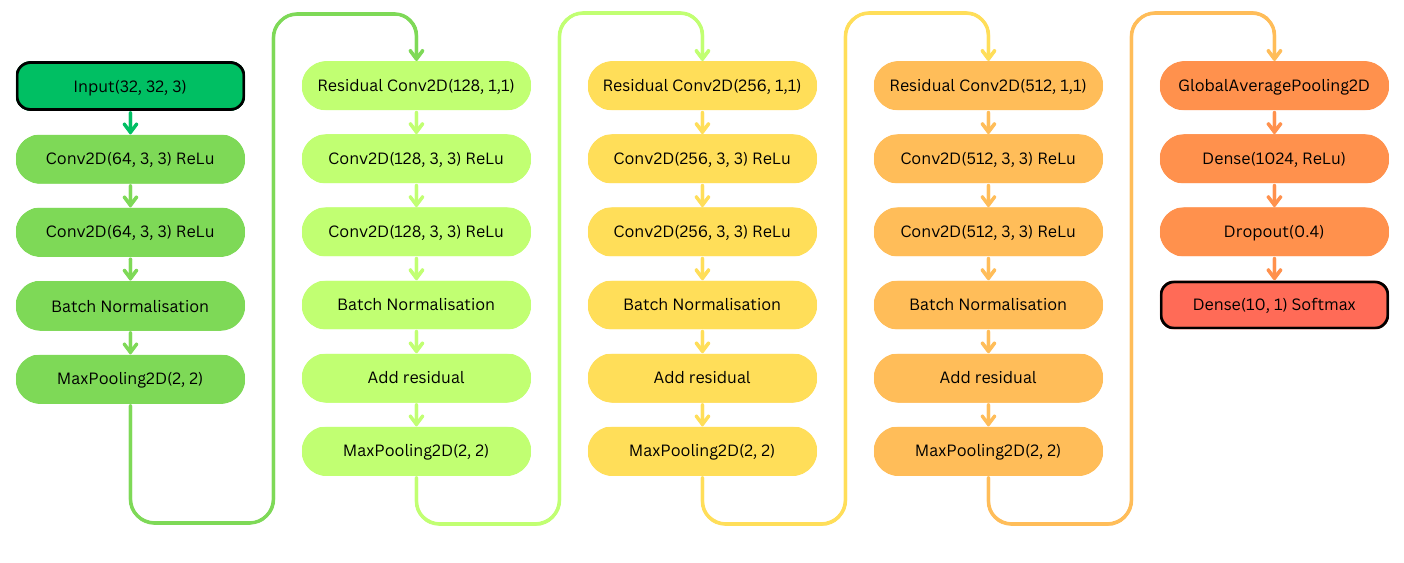
\includegraphics[width=\textwidth, height=0.3\textheight]{improved student model diagram croppped.png}
    \caption{Structural flowchart of the Improved Student Model}
    \label{fig:improved model}
\end{figure*}

\begin{table*}[t]
\centering
\begin{tabular}{|L|L|L|L|L|L|L|L|L|}
\hline
\textbf{Model} & \textbf{Parameters (Million)} & \textbf{Epochs} & \textbf{Training Accuracy (\%)} & \textbf{Test Accuracy (\%)} & \textbf{Test Error (\%)} & \textbf{Median 10 Epoch Time (seconds)} & \textbf{Fine Tuned} & \textbf{Confusion Matrix Reflective} \\ \hline
ResNet50 & 48.8 & 10 & 76.95 & 67.13 & 32.87 & 82 & Y & Y \\ \hline
EfficientNet & 26.1 & 10 & 86.67 & 82.73 & 17.27 & 38.5 & Y & Y \\ \hline
VGG16 & 33.6 & 10 & 9.73 & 10.00 & 90.00 & 72.5 & Y & Y \\ \hline
Student Model & 19.0 & 10 & 91.83 & 76.84 & 23.16 & 18.5 & N & Y \\ \hline
Improved Student Model & 5.39 & 10 & 92.77 & 79.59 & 20.41 & 40.5 & N & Y \\ \hline
Improved Student Model & 5.39 & 50 & 98.29 & 82.98 & 17.02 & N/A & N & Y \\ \hline
Improved Student Model & 5.39 & 100 & 98.82 & 81.95 & 18.05 & N/A & N & Y \\ \hline
\end{tabular}
\caption{Performance comparison of all models}
\label{tab:model_performance}
\end{table*}

The ResNet50 model was fine tuned with the initial weights being imported from tensorflow after training on the imagenet dataset. After 10 epochsthe model presented a 76.95\% accuracy. The test accuracy was 67.13\% and the error rate a reciprocal 32.87\%. The confusion matrix meaningfully reflected this perfomance. While the accuracy and losses over epochs indicate that the model is needing additional epochs but learning has meaningfully occurred. 

The EfficientNet model was fine tuned  with the initial weights being imported from tensorflow after training on the imagenet dataset. After 10 epochs the model displayed an 86.67\% training accuracy. The testing accuracy was a reflective 82.73\% with reciprocal error rate of 17.27\%. The confusion matrix also reflects teh learning achieved, displaying a difficulty in differentiating cats from dogs. The accuracy and losses over epochs display a trend that the model is approaching convergence after the 10 epochs. 

The VGG16 model was fine tuned with the initial weights being imported from tensorflow after training on the imagenet dataset. After 10 epochs the model displayed a 9.73\% accuracy, alongside a test accuracy of 10.0\% and a error rate of 90.0\%. The confusion matrix characterises that the model has not been able to extract any features over 10 epochs. As sucht he model is guessing that all inputs are a ship. The loss over epochs graph indicates that the model has entered a local minima and would require a smaller learning rate and additional epochs to be able to converge. This is supported by the accuracy over epochs data. 

\subsection{Improved Model}
The improved student model was developed to take advantage of all the architectures presented within ResNet, VGG, and EfficientNet, by incorporating them into the initial student model. The implementation of such can be seen in figure \ref{fig:improved model}. Where a residual calculation is made before and after each convolution and the inclusion of global average pooling was adapted from ResNet, additional convolution blocks at greater sizes were adapted from VGG, and convolution size then tempered after consideration from EffecientNet. The total parameters has also decreased from the student model, lowering from approximately 19 million parameters to approximately 5.39 million parameters. This improved model boasts a 5 fold smaller amount of parameters in comparison to the next smalelst fine tuned model. 

The improved model was trained for 10 epochs, achieving a 92.77\% accuracy contrasted with a test accuracy of 79.59\% and an error rate of 20.41\%. This was reflected in the confusion matrix, where differentiating dogs from cats and deer from horses remains difficult. The accuracy and losses over epochs, both display an the models approach toward convergence.

The improved model was further trained until 50 epochs and then until 100 epochs. After 50 epochs the best performance can be seen. The model achieved a 98.29\% accuracy, contrasted against an 82.98\% test accuracy with an error rate of 17.02\%. The confusion matrix reveals that the predictive behaviour is the same as the 10 epoch version but with better outcomes. The accuracy and losses over epochs data reveals that the model converged between 40 and 50 epochs. This is characterised by the oscillation in losses and accuracy.

The improved model was then trained until 100 epochs. This model displays that convergence has occurred without meaningful improvement from the additional epochs. The accuracy has increased from that of the 50 epoch model, a 98.82\%, however the model also displays a decreased test accuracy of 81.95\%. This reduced performance is supported further by the increased test error of 18.05\% and reflective confusion matrix performance. The accuracy and losses over epochs graphs display this change through marginal improvements that oscillate.

\section{Code}
\label{sec:code}
Please find the code \href{https://github.com/Drackonack/DLF_Assignment_02}{here}.

\section{Conclusion}
\label{sec:conclusion}
This study demonstrates the potential of leveraging transfer learning to improve model performance on the CIFAR-10 dataset. By analyssing both the architecture and performance of fine tuned established CNN architectures, VGG, ResNet, and EffecientNet, an improved model was developed. 

As detailed in the results, the Improved Student Model showed remarkable progress over the initial student model. After just 10 epochs, the model achieved 92.77\% training accuracy and 79.59\% test accuracy, with an error rate of 20.41\%. Extending training to 50 epochs improved test accuracy to 82.98\% and test error rate to 17.02\%. However, after 100 epochs, the model’s accuracy increased to 98.82\%, but decreased test accuracy 81.95\%, highlighting the model's eventual convergence and potential overfitting.

In comparison, the EfficientNet model displayed strong performance, with a test accuracy of 82.73\% and a relatively low error rate of 17.27\% after 10 epochs. ResNet50 dispalyed middling erformance after 10 epochs, with a test accuracy of 67.13\%, though its higher parameter count and longer training time suggest opportunities for optimization. The VGG16 model performed poorly, with a test accuracy near 10\%, revealing the need for the model to be configured further for meaningful performance. This was considered out of scope for the practice of the comparitive study.

Overall, the improved model, drawing inspiration from the other more advanced architectures, outperformed both baseline and fine-tuned models in key metrics, demonstrating that combining strategies from VGG, ResNet, and EfficientNet offers promising results in image classification tasks. This improved model also outperforms the model developed for the CIFAR-10 dataset \cite{cifar10} achieving a 17.02\% error rate, an 0.98\% improvement in comparison to the 18\% error rate without data augmentation.

The improved model however, would beenfit from further exploration of regularisation methods or even hyperparameter tuning to ensure consistent performance across both training and test datasets. As evidenced from the decrease in test accuracy with longer training. 

The confusion matrices highlighted persistent challenges in distinguishing between certain classes, such as cats and dogs, suggesting that future work could further focus on incorporating additional feature extraction techniques. Additionally, exploring ensemble techniques or more advanced optimization strategies could help mitigate the performance drop observed at higher epochs, ensuring the model's robustness in real-world applications.


%-------------------------------------------------------------------------

%%%%%%%%% REFERENCES
{\small
\bibliographystyle{ieee_fullname}
\bibliography{egbib}
}

\end{document}